\chapter{Introduction to Curve Fitting}

\section{Introduction}
This lab will introduce calculations and plotting techniques using numpy arrays within Scientific Python.

\section{Fitting a Straight Line with Scientific Python}

\begin{figure}[htbp]
\begin{center}
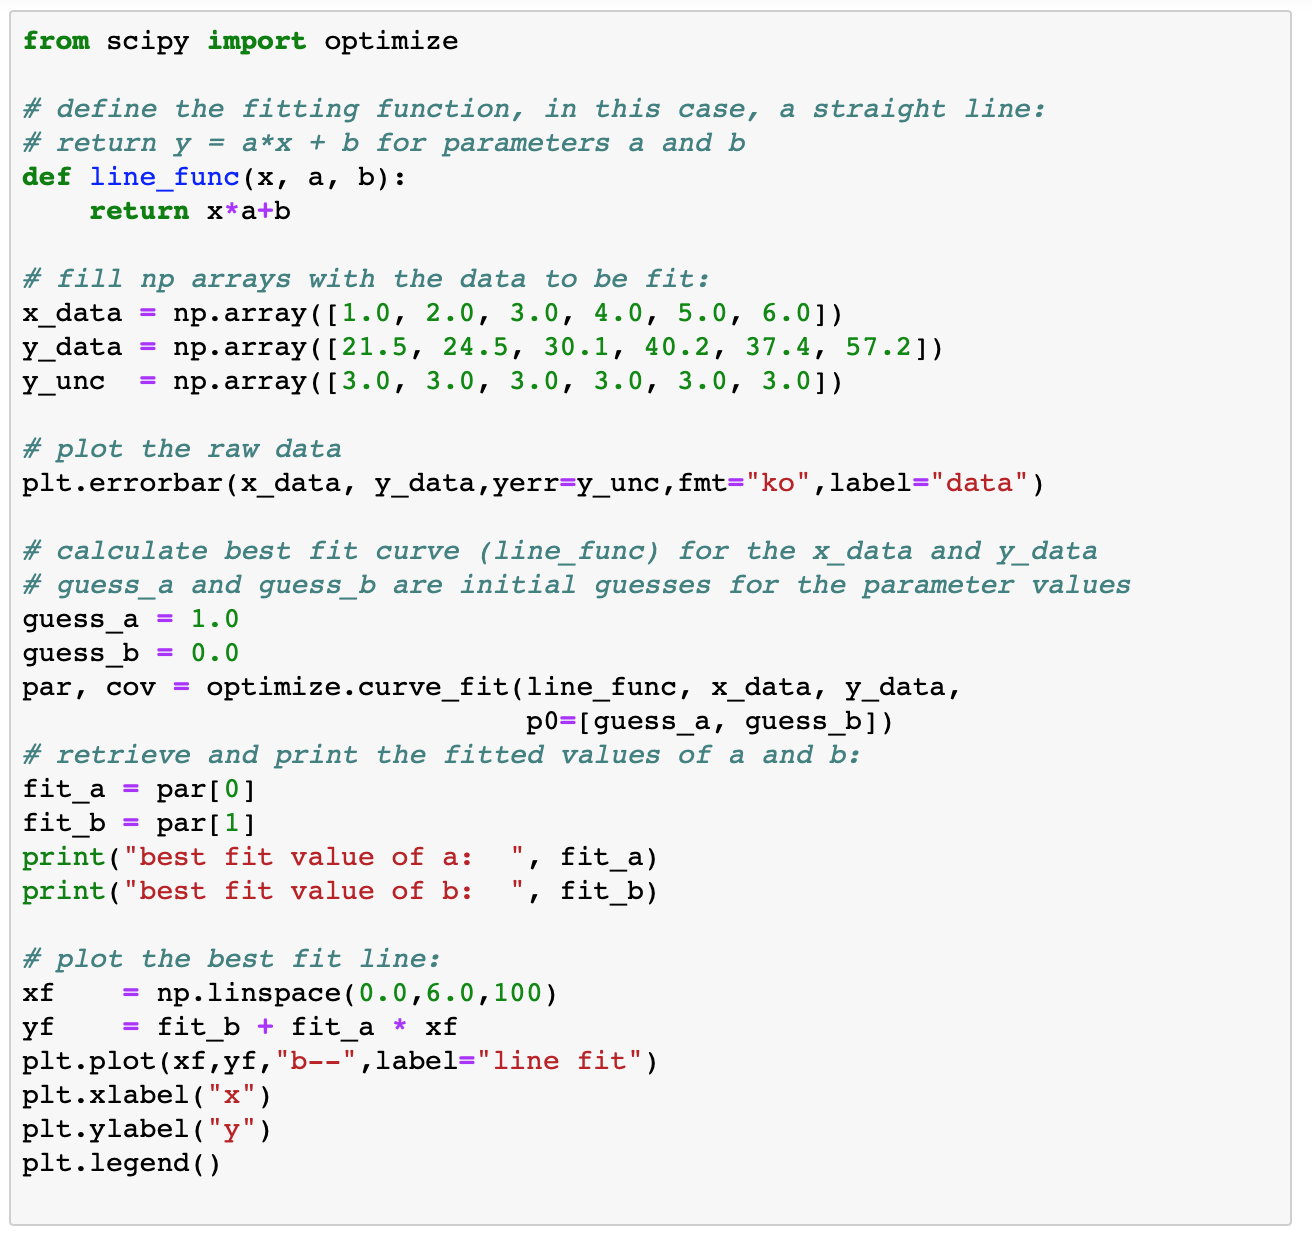
\includegraphics[width=0.65\textwidth]{figs/python/plotting/fit_code.png} \\
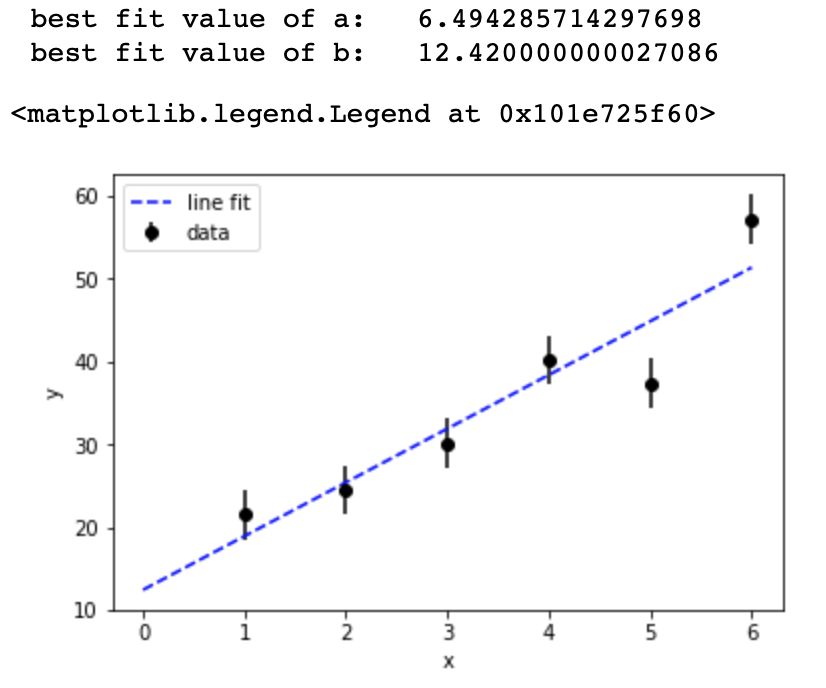
\includegraphics[width=0.65\textwidth]{figs/python/plotting/fit_out.png} \\
\caption{Example fitting data to linear relationship.}
\label{fig:plotsin}
\end{center}


\begin{figure}[htbp]
\begin{center}
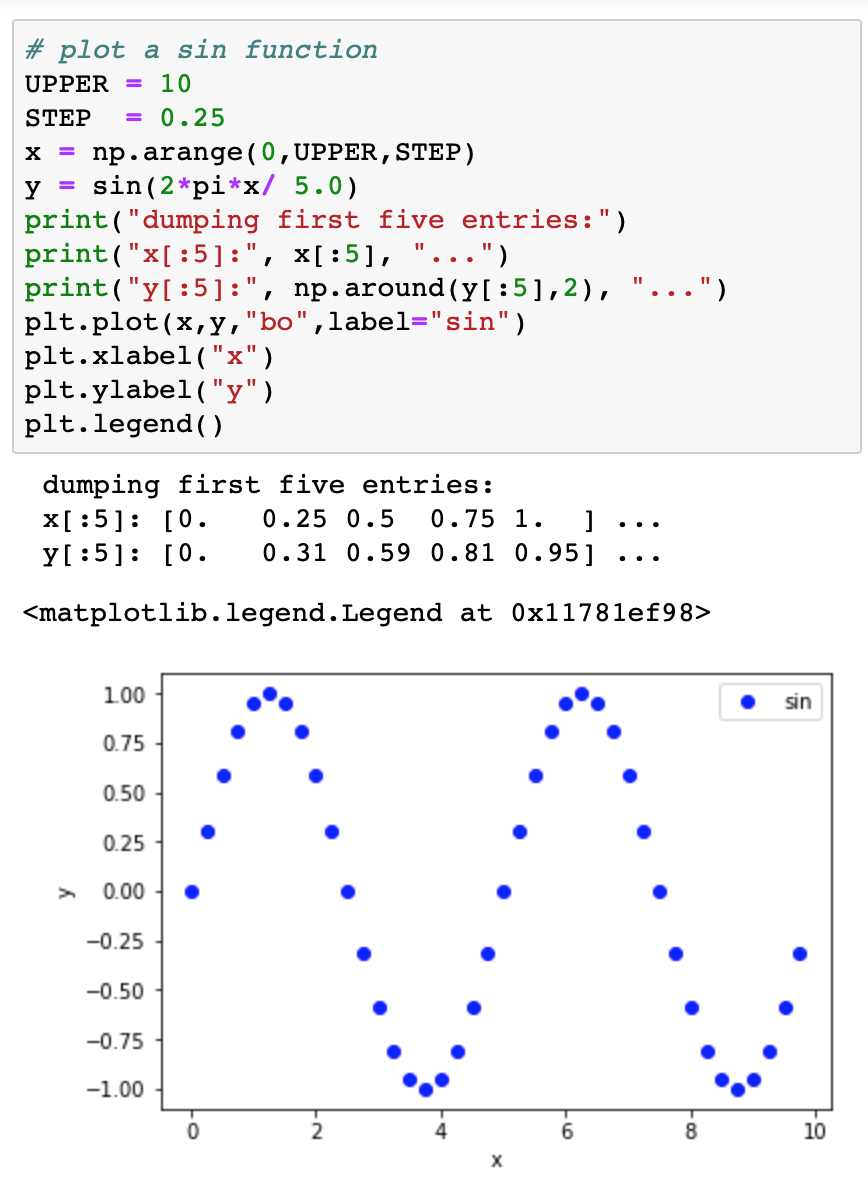
\includegraphics[width=0.65\textwidth]{figs/python/plotting/plotting.png} 
\caption{Circuit for verifying Ohm's law as a (a) circuit diagram, and (b) implemented using your lab equipment.}
\label{fig:plotsin}
\end{center}

\begin{table}
\caption{Sample data for a voltage measurement subject to high frequency noise.}
\label{tbl:hfnoiseeg}
\begin{center}
\begin{tabular}{lll}
$t~(\rm s)$ & $v~(\rm V)$ & $n$ \\
0.4  & 0.25  &  2.8 \\
1.1  & 2.37  &  7.3 \\
1.4  & 1.69  &  9.7 \\
1.9  & 0.93  &  1.3 \\
2.5  & -1.0  &  6.2 \\
3.0  & 0.95  &  4.8 \\
3.4  & 1.22  &  6.9 \\
4.1  & 0.54  &  4.0 \\
4.4  & 0.37  &  1.9 \\
4.8  & 0.13  &  4.0 \\
5.5  & -2.04  &  9.5 \\
6.2  & -2.06  &  8.7 \\
6.5  & -0.81  &  2.3 \\
7.0  & -0.95  &  5.3 \\
7.5  & 0.98  &  9.7 \\
7.9  & 0.27  &  8.3 \\
8.5  & -0.81  &  0.1 \\
9.0  & -0.59  &  5.1 \\
9.4  & -0.37  &  4.4 \\
9.9  & 0.56  &  9.9 \\
\end{tabular}
\end{center}
\end{table}

